\documentclass[10pt,letterpaper]{article}
%\usepackage[T1]{fontenc}
%\usepackage[utf8]{inputenc}
\usepackage{ragged2e,booktabs,multirow}
\usepackage{caption,capt-of}
\usepackage{graphicx}
\usepackage{array}
\renewcommand{\thetable}{S\arabic{table}}
\renewcommand{\thefigure}{S\arabic{figure}}

\newcolumntype{M}[1]{>{\begin{varwidth}[t]{#1}}l<{\end{varwidth}}}

\RequirePackage[LY1]{fontenc}

\renewcommand{\rmdefault}{ptm}
\renewcommand{\sfdefault}{phb}
\renewcommand{\ttdefault}{pcr}

%\RequirePackage[LY1,mtbold]{mathtime}
\def\helvetica{\fontfamily{phv}\selectfont}
\def\helveticaitalic{\fontfamily{phv}\itshape\selectfont}
\def\helveticabold{\fontfamily{phv}\bfseries\selectfont}
\def\helveticabolditalic{\fontfamily{phv}\bfseries\itshape\selectfont}
\def\helveticacn{\fontfamily{phv}\fontseries{mc}\fontshape{n}\selectfont}
\def\helveticacnitalic{\fontfamily{phv}\fontseries{mc}\fontshape{sl}\selectfont}
\def\helveticacnbold{\fontfamily{phv}\fontseries{bc}\fontshape{n}\selectfont}
\def\helveticacnbolditalic{\fontfamily{phv}\fontseries{bc}\fontshape{sl}\selectfont}

\title{Phylotyper: {\it In silico} predictor of molecular subtypes from gene sequences \\ \large Supplementary Information}
\author{Matthew D. Whiteside, Chad R. Laing and Victor P.J. Gannon}
\date{ }


\begin{document}
 
%\maketitle
 
\tableofcontents

\clearpage

\section{Supplementary Figures}

\subsection{Supplementary Figure S1}

\begin{figure}[h!]
\centering
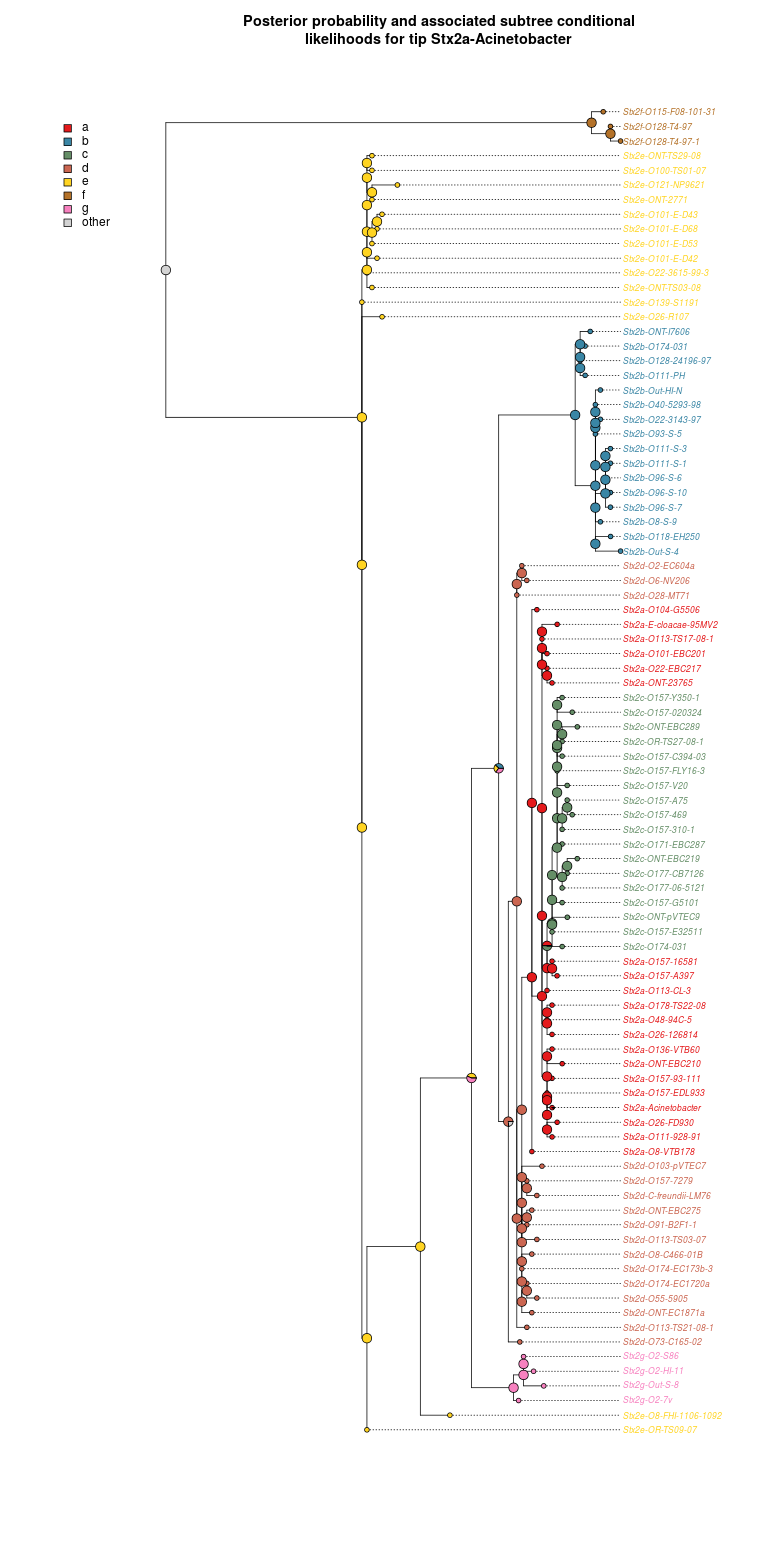
\includegraphics[scale=0.5]{sfig01.png}
\caption{Stx2 Phylogenetic tree showing the Phylotyper marginal likelihoods as pie charts. This output is provided to the user.}
\end{figure}

\clearpage

\section{Supplementary Tables}

\subsection{Supplementary Table S1}

\begin{minipage}{\linewidth}
\captionof{table}{Subtype Schemes in Phylotyper}
\medskip
\begin{tabular}{@{}llll@{}}\toprule Name &
Description & Species & Loci\\\midrule
stx1 & Shiga-toxin 1 subtype & {\it E. coli} & 2 \\
stx2 & Shiga-toxin 1 subtype & {\it E. coli} & 2\\
eae & Intimin subtype & {\it E. coli} & 1\\
flic & H-serotype based on flagellin gene; fliC & {\it E. coli} & 1\\
wz & O-serotype based on the wzy and wzx genes & {\it E. coli} & 2\\\bottomrule
\end{tabular}\par
\bigskip

\end{minipage}

\bigskip

\subsection{Supplementary Table S2}

Table S2 contains performance metrics from a leave-one-out cross-validation analysis comparing Phylotyper and a top-BLAST hit approach.  The analysis examines the four \textit{E. coli} schemes available in Phylotyper. In this multi-class analysis, precision, recall and F$_{1}$ score are calculated for each individual class provided that at least one instance of the class is in the training set.  The individual class positive and negatives are summed to calculate an overall precision, recall and F$_{1}$ score for the scheme.

\begin{minipage}{\linewidth}
\setlength{\tabcolsep}{4pt}
\captionof{table}{Leave-One-Out Cross Validation Results}
\medskip
\begin{tabular}{@{\extracolsep{4pt}}llll>{\centering}m{1.6cm}lll@{}}
\toprule 
\multirow{2}{*}{Scheme} & \multicolumn{4}{c}{Phylotyper} & \multicolumn{3}{c}{Sequence-similarity}\\
\cline{2-5}\cline{6-8}
& Precision & Recall & F$_{1}$ Score & Run-time (s) $^{1}$ & Precision & Recall & F$_{1}$ Score \\
\midrule
{\it E. coli} Stx1 & 1.00 & 0.94 & 0.97 & 6 & 0.94 & 0.94 & 0.94\\
{\it E. coli} Stx2 & 1.00 & 0.99 & 0.99 & 32 & 0.93 & 0.93 & 0.93\\
{\it E. coli} Intimin & 1.00 & 0.98 & 0.99 & 17 & 0.99 & 0.98 & 0.99\\
{\it E. coli} H-serotype & 0.99 & 0.98 & 0.98 & 16 & 0.96 & 0.85 & 0.90\\
{\it E. coli} O-serotype & 1.00 & 0.61 & 0.75 & 67 & 1.00 & 0.36 & 0.53\\\bottomrule
\end{tabular}\par
\bigskip
Formula:
\begin{enumerate}
\item $Precision = TP / (TP + FP)$
\item $Recall = TP / (TP + FN)$
\item $F_{1}~score = 2*Precision*Recall/(Precision + Recall)$
\end{enumerate}
$TP = True~Positive,~~FP = False~Positive,~~FN = False~Negative$
\par
\bigskip
$^{1}$ Run-time is for an {\it Escherichia coli} genome containing a non-identical subtype gene which triggers the full phylotyper pipeline.

\end{minipage}

\end{document}
